\documentclass[1p]{elsarticle}

\usepackage{lineno,hyperref}
\modulolinenumbers[5]

\journal{Journal of \LaTeX\ Templates}

%%%%%%%%%%%%%%%%%%%%%%%
%% Elsevier bibliography styles
%%%%%%%%%%%%%%%%%%%%%%%
%% To change the style, put a % in front of the second line of the current style and
%% remove the % from the second line of the style you would like to use.
%%%%%%%%%%%%%%%%%%%%%%%

%% Numbered
%\bibliographystyle{model1-num-names}

%% Numbered without titles
%\bibliographystyle{model1a-num-names}

%% Harvard
%\bibliographystyle{model2-names.bst}\biboptions{authoryear}

%% Vancouver numbered
%\usepackage{numcompress}\bibliographystyle{model3-num-names}

%% Vancouver name/year
%\usepackage{numcompress}\bibliographystyle{model4-names}\biboptions{authoryear}

%% APA style
\bibliographystyle{model5-names}\biboptions{authoryear}

%% AMA style
%\usepackage{numcompress}\bibliographystyle{model6-num-names}

%% `Elsevier LaTeX' style
%\bibliographystyle{elsarticle-num}
%%%%%%%%%%%%%%%%%%%%%%%

% ---------------------
% Pacotes OBRIGATÓRIOS
% ---------------------
%\usepackage{lmodern}				% Usa a fonte Latin Modern			
\usepackage[T1]{fontenc}			% Selecao de codigos de fonte.
\usepackage[utf8]{inputenc}		% Codificacao do documento (conversão automática dos acentos)
%\usepackage{lastpage}			% Usado pela Ficha catalográfica
%\usepackage{indentfirst}			% Indenta o primeiro parágrafo de cada seção.
\usepackage{color}			     	% Controle das cores
\usepackage{graphicx}	         % Inclusão de gráficos
\usepackage{epsfig,subfig}		% Inclusão de figuras
\usepackage{microtype} 			% Melhorias de justificação
% ---------------------

% ---------------------
% Pacotes ADICIONAIS
% ---------------------
\usepackage{lipsum}						% Geração de dummy text
\usepackage{amsmath,amssymb,mathrsfs, amsthm}	% Comandos matemáticos avançados 
\usepackage{setspace}  					% Para permitir espaçamento simples, 1 1/2 e duplo
\usepackage{verbatim}					% Para poder usar o ambiente "comment"
\usepackage{tabularx} 					% Para poder ter tabelas com colunas de largura auto-ajustável
\usepackage{afterpage} 					% Para executar um comando depois do fim da página corrente
\usepackage{url} 						% Para formatar URLs (endereços da Web)
\usepackage{todonotes}  		% Lista de afazeres To-dos
\usepackage{enumitem}					% Fazer enumerações por letras ou números nos itens
\usepackage{float}
\usepackage{longtable}					% Tabelas que se estendem por mais de uma página

% Configura o ambiente de teoremas, definições etc.

\theoremstyle{definition} 
\newtheorem{teor}{Teorema}%[section]
\newtheorem{defi}[teor]{Definição}
\newtheorem{lema}[teor]{Lema}
\newtheorem{supo}[teor]{Suposição}
\newtheorem{exemplo}[teor]{Exemplo}
\newtheorem{prop}[teor]{Proposição}


\begin{document}
	
\listoftodos

\begin{frontmatter}

\title{Medidas condicionais de risco através da teoria do valor extremo\tnoteref{mytitlenote}}
\tnotetext[mytitlenote]{Fully documented templates are available in the elsarticle package on \href{http://www.ctan.org/tex-archive/macros/latex/contrib/elsarticle}{CTAN}.}

%% Group authors per affiliation:
%\author{Rafael Felipe Bressan\fnref{myfootnote}\corref{correspondente}}
%\address{Avenida Madre Benvenuta, 2007 - Santa Mônica Florianópolis - SC 88035-901}
%\fntext[myfootnote]{Depto. de Economia/Esag/UDESC}

%% or include affiliations in footnotes:
\author[mymainaddress,mysecondaryaddress]{Elsevier Inc}
\ead[url]{www.elsevier.com}

\author[mymainaddress]{Rafael Felipe Bressan\corref{mycorrespondingauthor}\fnref{myfootnote}}
\cortext[mycorrespondingauthor]{Corresponding author}
\ead{rafael.bressan@edu.udesc.br}
\fntext[myfootnote]{Depto. de Economia/Esag/UDESC}

\address[mymainaddress]{Avenida Madre Benvenuta, 2007 - Santa Mônica Florianópolis - SC 88035-901}
\address[mysecondaryaddress]{360 Park Avenue South, New York}

\begin{abstract}
This template helps you to create a properly formatted \LaTeX\ manuscript.
\end{abstract}

\begin{keyword}
\texttt{elsarticle.cls}\sep \LaTeX\sep Elsevier \sep template
\MSC[2010] 00-01\sep  99-00
\end{keyword}

\end{frontmatter}

\linenumbers

\section{Introdução}

\paragraph{A medição do risco de mercado} ao qual os portfólios dos investidores está sujeito é objeto de devoção de esforços tanto por parte das instituições e investidores em geral como por parte dos reguladores. Instituições financeiras em todo o mundo, de acordo com suas regulações locais e com os princípios de Basileia (\emph{Basel Comittee on Banking Supervision} - BCBS do Banco de Compensações Internacionais - BIS\footnote{http://www.bis.org/bcbs/index.htm?m=3\%7C14}) para aquelas que o seguem (o Brasil é um desses países)  são obrigadas a reservar uma parcela de seu capital como provisionamento contra flutuações adversas do mercado em seus portfólios de investimento, como forma de mitigar seu risco de insolvência.

Instituições financeiras - IF - devem manter seu risco de insolvência controlado, e a percepção externa deve ser tal que não haja desconfiança do público em geral com a habilidade da instituição em controlar este risco. Confiança é a palavra chave destas instituições e portanto, também aos reguladores. Se a confiança se esvai e a percepção de risco é elevada, rapidamente uma crise de liquidez pode surgir, com depositantes sacando seus recursos e outras fontes de \emph{funding} também sendo limitadas. Em tal situação, é natural o banco (ou IF em geral) buscar o mercado para vender seus ativos e levantar os recursos necessários. É nesse momento que uma crise de liquidez pode levar a uma crise de solvência, não há garantias que no mercado aberto, os ativos do banco serão justamente avaliados e arrematados. A crise financeira de 2008 e 2009 ainda está na memória dos agentes.

Uma importante característica das séries de retornos financeiros é sua alta volatilidade, não constante e tampouco seguindo a distribuição Normal. Assim, eventos extremos, e neste caso estamos interessados em perdas de grande magnitude, acontecem com uma frequência alta demais para serem descartadas como apenas \emph{outliers}, e portanto passaram a atrair a atenção dos participantes do mercado, entre eles os investidores e também os reguladores. Estas observações induziram uma gama enorme de estudos, práticos e teóricos, voltados a explicar o comportamento dos retornos de séries financeiras e modelar de forma adequada as caudas da distribuição destes retornos. Não somente estes estudos são de grande relevância para o gerenciamento de risco nas instituições financeiras, como também são obrigatórios segundo o acordo de Basileia, uma vez que este requer o cálculo do Valor em Risco - VaR, para então a instituição poder projetar o seu nível requerido de capital. 

De acordo com os princípios de Basileia III, \cite{BankingSupervision2011, BankingSupervision2013, BankingSupervision2014}, as instituições financeiras supervisionadas pelos Bancos Centrais devem manter \emph{buffers} de capital contra riscos de mercado, crédito, liquidez, entre outros. Dentro dos riscos de mercado, as duas formas mais usuais de fazer a quantificação destes são os métodos de Valor em Risco - VaR e o \emph{Expected Shortfall} - ES. Este último relacionado ao primeiro, sendo definido como o valor esperado das perdas que excedem o valor VaR calculado para um determinado nível de confiança.
\todo{Percentuais de VaR por Basileia}
\todo{Existem penalidades regulatórias para as IF em que seu modelo VaR permite um número maior de perdas do que seria estimado pelo modelo. Verificar onde nos princípios de Basileia}

VaR é um quantil alto $\alpha$ da distribuição de perdas de um ativo ou portfólio em um determinado período de tempo, ao passo que ES é o valor esperado das perdas que excedem VaR, para um mesmo nível de confiança $\alpha$ e período.

O método VaR para cálculo de risco de mercado ao qual um portfólio está sujeito foi primeiramente introduzido através de \cite{RiskMetrics1995}, uma metodologia adotada pelo banco J. P. Morgan. Vem desde então sendo amplamente adotado pela indústria financeira e largamente estudado pela academia. Inúmeras variantes do modelo foram propostas e continuam sendo utilizadas com o passar dos anos. Para o cálculo do VaR é necessária uma suposição acerca da distribuição dos retornos, e por conseguinte do comportamento da cauda desta.

As variações na metodologia original de estimação do VaR surgem principalmente em função de críticas a abordagem proposta, a qual inclui a suposição de retornos independentes e igualmente distribuídos, covariâncias constantes entre os ativos de um portfólio e a distribuição normal dos retornos.

Por meio de dois artigos \cite{Artzner1997} e \cite{Artzner1999}, foi introduzido na literatura o conceito de medida coerente de risco. Para uma medida ser considerada coerente, primeiramente foram introduzidas quatro propriedades cunhadas através de axiomas, as quais estas medidas deveriam possuir, invariância a translação,	sub-aditividade, homogeneidade positiva, e monotonicidade.

VaR especificamente não possui a propriedade da sub-aditividade para alguns casos, sendo esta uma das grandes críticas ao VaR. Para contornar este fato, \cite{Acerbi2002} propõe o \emph{Expected Shortfall} e comprovam que este é uma medida coerente de risco. Além de ser coerente, o ES possui uma segunda vantagem com relação ao VaR, considerando que o ES nos informa uma medida de tendência central do tamanho das perdas que excedem o valor do quantil VaR. Ou seja, o VaR nos informa apenas que uma proporção $\alpha$ das perdas serão menores que a medida, mas nada nos informa se esta perda extraordinária de fato ocorrer. Mesmo sendo criticado e demonstradamente uma medida não coerente de risco, o VaR continua a ser amplamente utilizado, mesmo que agora em conjunto com o ES. 

%Mais recentemente o Comitê de Supervisão Bancária de Basileia tem se proposto a adotar o \emph{Expected Shortfall} como medida de risco de mercado. \cite{BankingSupervision2013a}. O Comitê cita a grande importância da escolha da medida de risco e sua calibração, e portanto estas são relevantes para as decisões de política do Banco. Entre as dificuldades encontradas pelo VaR estão mais notadamente sua inabilidade em estimar o "risco de cauda" da distribuição de perdas, uma vez que VaR não leva em conta a distribuição das perdas acima do valor de corte.

%Desta forma, foi decidido que o ES seria a medida de risco favorita para a abordagem pelo banco chamada de modelos internos. Ou seja, os bancos supervisionados devem utilizar o ES para o cálculo do risco de mercado a que estão sujeitos em seus modelos internos. O comitê também se decidiu por um nível de confiança de 97,5\% para o ES, em contraposição a 99\% para o VaR. O comitê espera que esta abordagem para o cálculo da medida de risco de mercado trará benefícios se comparada a antiga abordagem pelo Var, entre elas um modelo com resultados mais estáveis e menor sensibilidade a observações extremas (\emph{outliers}).

\paragraph{Teoria do valor extremo} EVT da sigla em inglês, é um ramo da estatística que lida diretamente com eventos raros, extremos. Seu objetivo é modelar o comportamento assintótico de eventos que se distanciam muito da mediana de uma distribuição. Justamente por esta característica, a EVT está sendo utilizada para modelar riscos que possuem distribuição com caudas longas, um dos fatos estilizados bem conhecidos sobre retornos de ativos financeiros.

Ao utilizar a EVT, e mais especificamente o método conhecido como \emph{peaks over treshold} – POT, se está interessado em modelar apenas a parte da cauda da distribuição das perdas de um ativo financeiro maiores que um determinado valor de limiar \emph{u}. É da modelagem desta cauda, portanto, que se calculam as estimativas de risco $VaR_\alpha$.

\todo{incluir as diversas literaturas sobre a aplicação da evt ao VaR}

\cite{McNeil2000}
\cite{Longin2000} \emph{stress test} utilizando evt
\cite{Wong2003} um estudo sobre as implicações da precisão do modelo VaR no gerenciamento do risco de mercado em bancos
\cite{Berkowitz2002} precisão dos modelos em bancos comerciais
\cite{Bystroem2004}
\cite{Gencay2004}
\cite{Kuester2006} comparação entre diversos modelos VaR
\cite{Herrera2013}
\cite{Rocco2014} uma revisão sobre o uso da evt em finanças
\cite{Karmakar2014}
\cite{Chavez-Demoulin2016}
\cite{Karmakar2016} aplicação do modelo evt condicional a retornos intra-diários
\cite{OBrien2017} avaliação dos modelos de risco de bancos no pré, durante e pós crise financeira de 2008

\section{Modelando caudas e medidas de risco associadas com EVT}
\label{sec:caudas}

Considere uma amostra de uma variável aleatória - \emph{va} - cujas observações sejam independentes e igualmente distribuídas - \emph{iid}, $X_i$, com $i\in \mathbb{N}$, que representem as perdas financeiras de um determinado ativo, com uma função de distribuição - \emph{df} - desconhecida $F(x) = P(X_i \leq x)$.
Seja \emph{u} um valor de limiar a partir do qual perdas acima deste valor sejam consideradas extremas. Os valores de excesso serão, portanto, $X_i - \emph{u}$.

A EVT está interessada em investigar o comportamento da distribuição dos máximos desta \emph{va} dados por $M_n = \max (X_1, \ldots , X_n)$ para vários valores de $n$ e a medida que $n\rightarrow \infty$. A sequência $M_n$ é chamada de máximos em bloco e foi demonstrado através do conhecido teorema de Fisher-Tippett-Gnedenko, \cite{Fisher1928}, \cite{Gnedenko1941, Gnedenko1943}, que a única distribuição para a qual $M_n$ converge com $n\rightarrow \infty$ é a distribuição de valores extremos generalizada. Se esta distribuição de valores extremos generalizada - GEV - for denotada por $H_\xi$, com $\xi$ um parâmetro da distribuição, então se diz que $F \in MDA(H_\xi)$, $F$ pertence ao domínio de máxima atração de $H_\xi$.


\begin{defi}[GEV] \label{defi:GEV}
	Distribuição de valores extremos generalizada, é definida por sua função densidade de probabilidade - pdf - a qual é dada por:
	
	\begin{equation}
	\label{eq:GEV}
	H_\xi(x) = 
	\begin{cases}
	exp(-(1+\xi x)^{-\frac{1}{\xi}}), & \xi \neq 0,\\
	exp(-e^{-x}), & \xi = 0,\\
	\end{cases}
	\end{equation}
\end{defi}

O parâmetro $\xi$ é conhecido como parâmetro de forma da distribuição e dependendo deste valor tem-se diferentes tipos de distribuição (casos particulares da GEV). Quando $\xi=0$ a distribuição resultante é uma Gumbel, quando  $\xi>0$ uma Fréchet surge, e por fim quando $\xi<0$ tem-se uma Weibull.

Para as aplicações financeiras não necessitamos calcular a qual $MDA$ pertencem nossas distribuições contínuas, bastando saber que basicamente todas as distribuições de utilidade prática estão contidas em $MDA(H_\xi)$ para algum valor de $\xi$ \cite[p. ~139]{McNeil2015}.

\subsection{Excessos acima de um limiar}
\label{sec:excess}

O método POT para calcular a função de distribuição dos valores que excedem um determinado limiar de um conjunto de dados vem sendo empregado no mundo financeiro para ajustar as caudas das distribuições de retornos, ou perdas, dos ativos. Este método é preferido a teoria clássica de valores extremos (e.g. máximos em bloco), pois, desperdiça uma quantidade menor de dados da série original. Qualquer valor que exceda o limiar pré-determinado é considerado na distribuição dos excessos. Esta é definida como.

\begin{defi}[Distribuição dos excessos] \label{defi:excess}
	Seja \emph{X} uma variável aleatória com função de distribuição \emph{F}. A distribuição dos excessos sobre um limiar \emph{u} tem a seguinte função de distribuição:
	
	\begin{equation}
	\label{eq:excessdist}
	F_u(x)=P(X-u \leq x | X > u)=\frac{F(x+u)-F(u)}{1-F(u)}
	\end{equation}
	para $0 \leq x < x_F-u$, onde $x_F \leq \infty$ é o limite direito da distribuição \emph{F}.
\end{defi}

Uma importante distribuição que surge na modelagem dos excessos sobre um limiar é a distribuição gereralizada de Pareto – GPD, que segue.

\begin{defi}[GPD] \label{defi:GPD}
	Distribuição de Pareto Generalizada é definida por sua função de distribuição:
	\begin{equation}
	\label{eq:GPD}
	G_{\xi,\psi}(x) = 
	\begin{cases}
	1- \left(1+ \frac{\xi x}{\psi} \right)^{-\frac{1}{\xi}}, & \xi \neq 0,\\
	1-exp\left(-\frac{x}{\psi}\right), & \xi = 0,\\
	\end{cases}
	\end{equation}
	onde $\psi > 0$, e $x\geq 0$ quando $\xi  \geq 0$ ou $0 \leq x \leq -\psi / \xi$ quando $\xi < 0$.
\end{defi}

Os parâmetros $\xi$ e $\psi$ são conhecidos respectivamente como parâmetros de forma e escala da distribuição. A GPD tem papel fundamental na teoria de valor extremo em função do teorema de Pickands-Balkema-de Haan, \cite{Pickands1975} e \cite{Balkema1974}, pois estes demonstram que, para um valor suficientemente alto do limiar \emph{u}, a distribuição dos excessos $F_u(x)$ pode ser aproximada por uma GPD $G_{\xi,\psi}(x)$.

O que este teorema prova é que para distribuições as quais os máximos em bloco normalizados convergem para uma GEV (na forma da equação \eqref{eq:GEV}), então a distribuição dos excessos acima de um limiar destas mesmas distribuições convergem para uma GPD, dado um valor de limiar \emph{u} adequado. Como para fins práticos basicamente todas as distribuições contínuas de fato estão no $MDA(H_\xi)$ para algum valor de $\xi$, temos que a GPD é a distribuição a ser escolhida para modelar excessos acima de um limiar.

Ao se fazer esta suposição que a distribuição dos excessos \emph{é igual} a uma GPD, pode-se então, a partir dos dados de perdas, estimar os parâmetros de forma e escala e, portanto, modelar a cauda direita da distribuição de perdas de forma parametrizada com o auxílio da equação \eqref{eq:excessdist}. 


Dada a parametrização de uma GPD, é interessante saber o valor esperado desta distribuição, uma vez que esta medida de valor central fornece importante informação sobre a quantidade de risco que se está medindo, assim como a informação de que a própria distribuição foi ajustada aos dados de forma satisfatória.

O valor esperado de uma variável aleatória não negativa pode ser computado através da integral de sua cauda, $P(X>x) = 1-P(X \leq x)$. A cauda da GPD é, para $\xi \neq 0$, $\left(1+\xi x / \psi \right)^{-1/ \xi}$.

Desta forma, o valor esperado de uma GPD, $G_{\xi,\psi}(x)$, converge para valores de $\xi<1$ e é dado pela seguinte equação:

\begin{equation}
\label{eq:meanGPD}
E\left[G_{\xi,\psi} (X) \right]=\frac{\psi}{1-\xi}
\end{equation}


\begin{defi}[função média dos excessos]
	\label{defi:meanexcess}
	A função média dos excessos de uma variável aleatória \emph{X} com média finita é dada por:

	\begin{equation}
	\label{eq:meanexcess}
	e(u)=E\left(X-u | X > u\right)
	\end{equation}
\end{defi}

Ou seja, a equação \eqref{eq:meanexcess} representa o valor esperado da função de distribuição dos excessos dada pela Definição \ref{defi:excess}. Ela representa a média de $F_u$ como uma função do limiar \emph{u}. Por vezes também é conhecida como função média de vida residual (\emph{mean residual life function}).

Para uma variável distribuída na forma de uma GPD, o parâmetro de escala é uma função linear em \emph{u} dado por $\psi(u)=\psi + \xi u$, \cite[Teorema 3.4.13(e)]{Embrechts1997}. Utilizando-se deste fato e da equação \eqref{eq:meanGPD} chegamos ao cálculo da função média dos excessos para uma GPD, dada por:

\begin{equation}
\label{eq:eu}
e(u)=\frac{\psi+\xi u}{1-\xi}
\end{equation}
onde $0 \leq u < \infty$ se $0 \leq \xi <1$ e $0 \leq u \leq -\psi / \xi$ se $\xi < 0$. É possível observar que de fato a função média dos excessos em uma GPD é linear em \emph{u}. Esta é uma característica importante de uma GPD e que pode ser utilizada para auxiliar a escolha de um valor adequado do limiar \emph{u} de tal forma que a suposição de convergência $F_u(x) \rightarrow G_{\xi, \psi}(x)$ seja válida.

Assim, quando da análise de uma determinada distribuição de perdas \emph{F} e deseja-se ajustar a cauda desta, ou seja, ajustar as perdas acima de um dado valor limiar \emph{u} a uma GPD $G_{\xi, \psi}(x)$ é necessário primeiramente determinar um valor adequado de \emph{u} que garanta a suposição de convergência. Um método frequentemente utilizado é o gráfico da função média dos excessos com relação a \emph{u}. Analisando este gráfico, escolhe-se o menor valor de \emph{u} para o qual a partir deste ponto a relação $e(u) \text{ vs } u$ torna-se linear.

Deseja-se o menor valor de \emph{u} para o qual a relação é linear pois, mesmo o método POT implica em grande perda de dados da série temporal, já que apenas os valores acima deste limiar são utilizados para fazer a estimação dos parâmetros $\xi$ e $\psi$ da GPD. Portanto, existe um \emph{trade-off} na escolha do valor limiar \emph{u}, escolhendo um valor muito baixo obtém-se uma boa quantidade de dados para estimar os parâmetros da GPD, mas a própria distribuição resultante não será GPD, uma vez que não estaremos trabalhando na região onde a relação $e(u) \text{ vs } u$ é linear, e portanto os parâmetros estimados serão viesados. Por outro lado, um valor limiar muito alto impõe o custo de trabalhar com poucos dados para fazer a estimação dos parâmetros da distribuição e por conseguinte, os erros padrões dessas estimativas serão elevados.

Considerando este \emph{trade-off}, uma saída é buscar minimizar o erro quadrado médio - MSE (\emph{mean squared error}) do parâmetro estimado. A medida MSE pode ser decomposta entre a soma do quadrado do viés com a variância do estimador, idealmente deseja-se ter viés zero e variância mínima. Na impossibilidade de tal realização, um estimador relativamente eficiente é aquele que possui o menor MSE. Em \cite[seção 5.2.5, p. ~139]{McNeil2015} é explorada através de simulação de Monte Carlo esta relação entre a escolha do limiar \emph{u} e o MSE do parâmetro $\xi$ obtido através do método POT e também da própria medida de risco $VaR_{99\%}$. Chegam a conclusão que uma escolha de limiar tal que o número de excessos a este fique em torno de 100 observações é o ideal, e mais importante, a partir destas 100 observações o MSE é relativamente robusto, se elevando lentamente a partir de seu valor mínimo.

\subsection{Estimando o VaR}
\label{sec:var}

Através da modelagem da cauda da distribuição \emph{F} de perdas por uma GPD, é possível calcular a medida de risco $VaR_\alpha$ em função dos parâmetros da GPD estimada e também fazendo uso da distribuição empírica de \emph{F}.

Sob a suposição de convergência a cauda da distribuição \emph{F}, $\bar{F}(x)$, para $x \geq u$ é dada por:

\begin{align}
\label{eq:Ftail}
\bar{F}(x) & = P(X>u)P(X>x|X>u) \nonumber \\
& = \bar{F}(u) P(X-u>x-u|X>u) \nonumber \\
& = \bar{F}(u)\bar{F}_u(x-u) \nonumber \\
& = \bar{F}(u)\left(1+\xi \frac{x-u}{\psi}\right)^{-1/\xi}
\end{align}

Aqui $x$ são os valores a serem observados das perdas, e portanto $x-u$ são as perdas em excesso ao limiar.

A equação \eqref{eq:Ftail} efetivamente separou a distribuição \emph{F}, ou melhor, sua cauda, em duas partes. A primeira parte, para valores menores que \emph{u}, não foi modelado analiticamente e portanto utiliza-se a distribuição empírica das perdas, aqui representada por sua cauda $\bar{F}(u)$, que nada mais é que o número observado de excessos de \emph{u} sobre o número total de observações da amostra.

A segunda parte é justamente a modelagem através de uma GPD com parâmetros $\xi$ e $\psi$ dado o limiar \emph{u}. Por esta modelagem paramétrica pode-se conhecer as probabilidades de cauda para valores de \emph{x} maiores que \emph{u}.

O quantil $\alpha$ é a inversa da função distribuição e retorna o valor para o qual um percentual $\alpha$ de observações da amostra é menor ou igual. Como se está trabalhando com a distribuição de perdas, $VaR_\alpha$ nada mais é que um quantil alto para o qual $\alpha \%$ das perdas devem ser menores ou iguais a este valor.

Como a equação \eqref{eq:Ftail} fornece a probabilidade de cauda, então esta é igual a $1- \alpha$ para um valor de $\alpha  \geq \bar{F}(u)$. O valor $1- \alpha$ é conhecido como a cobertura da medida de risco. Fazendo $\bar{F}(x)=1-\alpha$ na equação \eqref{eq:Ftail} o valor de \emph{x} representará $VaR_\alpha$ e basta manipular esta equação para encontrar $VaR_\alpha$ como função de $\bar{F}(u)$, $\alpha$ e dos parâmetros da GPD $\xi$ e $\psi$. Que garante a equação abaixo:

\begin{equation}
\label{eq:VaRGPD}
VaR_\alpha = q_\alpha(F) = u+\frac{\psi}{\xi}\left[ \left( \frac{1-\alpha}{\bar{F}(u)}\right)^{-\xi}-1 \right]
\end{equation}

Portanto, a medida de risco $VaR_\alpha$, para distribuições de perdas que tiveram suas caudas modeladas através de uma GPD da forma $G_{\xi, \psi(u)}$ com $\xi <1 \text{ e } \psi > 0$, pode ser calculada através da equação dada em \eqref{eq:VaRGPD}. A estimativa desta medida de risco será encontrada através das estimativas dos parâmetros da GPD, assim como do limiar utilizado e de uma medida empírica de $\bar{F}(u)$ que será o número de excessos verificados sobre o total de amostras. É claro que, ao se adotar esta estimativa para $\bar{F}(u)$ se está implicitamente supondo que o número de amostras na série de perdas é significativa, assim como o número de excessos verificados. Daí a importância de se utilizar um valor \emph{u} adequado, conforme explicitado na seção \ref{sec:excess}.

A estimativa de medida de risco desenvolvida nesta seção se qualifica como uma medida incondicional, no sentido que ela não depende do estado atual das coisas, mas sim de todo o histórico de eventos de forma uniforme. Em outras palavras, $VaR_\alpha$ derivado a partir da equação \eqref{eq:VaRGPD} é uma medida histórica de risco associado ao ativo em análise, entretanto, não leva em consideração se nos eventos mais recentes a volatilidade das perdas pode ser diferente do valor histórico.

De fato, uma das características marcantes das perdas (ou equivalentemente, dos retornos) dos ativos financeiros é o chamado \emph{clustering} de volatilidade, onde grandes volatilidades têm tendência a ficarem próximas ao longo da linha temporal. Em geral estes agrupamentos de volatilidades surgem a partir da autocorrelação destas, ou seja, a volatilidade em um período \emph{t} é dependente das volatilidades verificadas em períodos anteriores. Um modelo bastante encontrado na literatura que busca modelar estas dependências é o modelo ARCH e suas variantes como GARCH, propostos por \cite{Engle1982} e \cite{Bollerslev1986} respectivamente.

Assim, ao passo que as estimativas de risco desenvolvidas nesta seção são valiosas para prazos mais longos, ainda é necessário desenvolver um modelo que lide com o fato das autocorrelações de volatilidades das perdas e, portanto, com o fatos de a distribuição das perdas não ser independente e igualmente distribuída ao longo do tempo. O modelo proposto por \cite{McNeil2000} pode ser utilizado para encontrar a medida de risco $VaR_\alpha$ condicional que se deseja, ainda dentro da metodologia POT.

\subsection{Modelo eGARCH-POT}
\label{sec:egarchpot}

Ativos financeiros possuem características de autocorrelação, senão em seus retornos propriamente ditos, ao menos em suas volatilidades ou variações absolutas. Ou seja, dada uma grande variação no momento \emph{t} é de se esperar novamente uma grande variação, não necessariamente na mesma direção daquela anterior, para o momento \emph{t+1} e posteriores. Desta forma, medidas de risco incondicionais, conforme aquelas derivadas em \ref{sec:caudas} podem ser adequadas somente para horizontes temporais mais longos, pois implicitamente tomam em consideração os fatos mais recentes com o mesmo valor de predição que fatos mais longínquos.

Assim, pode-se trabalhar com um modelo semelhante ao proposto por \cite{McNeil2000} os quais fazem uma adequação dos retornos dos ativos a um modelo GARCH e posteriormente tratam os erros desta modelagem como \emph{iid} e portanto, a metodologia de POT pode ser aplicada. Este modelo pode ser entendido como um modelo condicional para medidas de risco pois, efetivamente, é levado em conta o estado atual da previsão para a média e principalmente para a volatilidade ao se calcular o $VaR_\alpha$. Desta forma a medida responde rapidamente às variações nos humores do mercado e pode sinalizar de forma ágil uma inadequação de capital reservado pela instituição financeira.

Além desta vantagem de cunho prático, a técnica possui uma atratividade teórica. O método POT deve ser aplicado a séries \emph{iid} que sabidamente não é o caso de perdas de ativos financeiros. Ao se utilizar a técnica POT nos resíduos padronizados de um modelo GARCH das perdas, o que se está realizando é uma pré-filtragem destas perdas que garante, ou chega próximo disto, que os resíduos deste modelo sejam \emph{iid} e portanto, aplicável a teoria de valor extremo. 

Primeiramente, neste artigo, diferentemente de \cite{McNeil2000} ou \cite{Karmakar2014}, foi estabelecido um mesmo modelo eGARCH para as perdas dos ativos subjacentes. Esta variação de GARCH foi proposta por \cite{Nelson1991} e busca, além de modelar a heterocedasticidade condicional da variância, também o chamado efeito alavancagem, onde retornos positivos e negativos possuem impactos diferenciados na volatilidade do ativo. O modelo adotado foi o eGARCH(2,1) e sua variância condicional é definida por:

\begin{align}
\label{eq:egarch}
\ln\sigma_t^2=&\omega+ \sum_{i=1}^{2}\left(\alpha_i Z_{t-i}+ \gamma_i(|Z_{t-i}|-E|Z_{t-i}|)\right)+ \beta_1 \ln\sigma_{t-1}^2
\end{align}
onde os coeficientes $\alpha_i$ capturam o efeito do sinal do erro, enquanto que os parâmetros $\gamma_i$ o efeito magnitude destes erros. O coeficiente $\beta_1$ continua a ser o chamado coeficiente garch. %O valor esperado do absoluto das inovações é calculado como segue:

%\begin{align}
%	E\left| Z_t\right|=&\int_{-\infty}^{\infty}|Z|f(z)dz
%\end{align}

Denotando $L_t$ como sendo a perda observada no período \emph{t}, $\mu_t$ e $\sigma_t$ são respectivamente a média e o desvio padrão condicionais, e seja $Z_t$ inovações \emph{iid} com média zero e desvio padrão unitário, então tem-se que:

\begin{equation}
\label{eq:loss}
L_t=\mu_t+\sigma_t Z_t
\end{equation}

Seja $F_L(l)$ a distribuição marginal de $L_t$, então $F_{L_{t+1}} | \mathcal{G}_t(l)$ é a distribuição preditiva da perda para o próximo período, onde $\mathcal{G}_t$ é o conjunto de informações disponíveis no período \emph{t}, incluindo-o. Portanto, para o cálculo de $VaR_\alpha$, se deseja encontrar o alfa-quantil na cauda de $F_{L_{t+1}} | \mathcal{G}_t(l)$. Este quantil $\alpha$ é o ínfimo \emph{l} tal que o valor da distribuição preditiva seja maior ou igual a $\alpha$. Ou seja:

\begin{align}
VaR_\alpha^t=&\inf\{l \in \mathbb{R}: F_{L_{t+1}} | \mathcal{G}_t(l) \geq \alpha\}
\end{align}

Veja, este é o preditor de $VaR_\alpha$ calculado com as informações até o período \emph{t}, inclusive. Este valor calculado deve ser comparado a perda realizada em \emph{t+1}, para testar uma possível violação.
Considerando que a distribuição de perdas é dada pela equação \eqref{eq:loss} e sabendo das propriedades de variáveis aleatórias e do operador de expectância, a expressão de $VaR_\alpha^t$ subsume a:

\begin{align}
\label{eq:varcond} 
VaR_\alpha^t=&\mu_{t+1}+\sigma_{t+1}z_\alpha 
\end{align}
onde $z_\alpha$ é o quantil $\alpha$ das inovações $Z_t$.

Dadas estas considerações, o modelo adotado segue um formato em dois estágios para ser implementado, como segue.
\begin{itemize}
	\item Ajustar um modelo eGARCH para os dados de perdas, sem fazer suposições sobre a distribuição de \emph{Z}. Deste modelo retira-se as estimativas de $\mu_{t+1}$ e $\sigma_{t+1}$ e calcula-se as inovações implícitas resultantes, através da equação \eqref{eq:loss}.
	\item Ao se considerar os resíduos padronizados como sendo as realizações da variável aleatória \emph{Z}, esta pode ter sua cauda ajustada a uma GPD utilizando-se o método descrito na seção \ref{sec:caudas}. Encontra-se por fim o valor de $z_\alpha$, com o qual é finalizado o cálculo $VaR_\alpha$ através da equação dada em \eqref{eq:varcond} para os valores de $\alpha$ iguais a 0,975 e 0,99.
\end{itemize}

Agora é necessário escolher um processo que modele a série temporal dada em \eqref{eq:loss}, ou seja, precisa-se especificar o comportamento de $\mu_t$ e $\sigma_t$. Por suposição, o comportamento destas variáveis é dependente de acontecimentos passados, contidos no conjunto de informações $\mathcal{G}_{t-1}$ . Pode-se estipular um modelo eGARCH(2,1) para a volatilidade condicional e um simples AR(1) para a média condicional. A ordem destes modelos foi escolhida como uma forma de compromisso entre parcimônia e o melhor ajuste dentre diversos outros modelos e ordens para os 6 ativos sob análise. Estes modelos eGARCH(2,1) e AR(1) para as volatilidades e médias condicionais respectivamente foram aqueles que, de forma geral, se ajustaram mais adequadamente as séries dadas.

Como critérios para a escolha deste modelo de filtro no primeiro estágio, deseja-se que as inovações $Z_t$, através de suas realizações na forma dos resíduos padronizados estimados no modelo possuam 2 características, ausência de autocorrelação serial em seus valores e nos seus quadrados.

Visando aplicar a teoria do valor extremo para o cálculo de $VaR_\alpha$, não são feitas maiores assunções acerca da distribuição das inovações, mas está implícito que esta pertence ao \emph{MDA} de uma GEV e portanto a distribuição de seus excessos sobre um limiar segue aproximadamente uma GPD.

O modelo completo para a medida condicional de risco $VaR_\alpha$ dada a distribuição de perdas $L_t$ de um ativo será, portanto:

\begin{align}
L_t=&\mu+ \phi_1 L_{t-1}+\epsilon_t \\
\epsilon_t=&\sigma_t Z_t\\
\ln\sigma_t^2=&\omega+ \sum_{i=1}^{2}\left(\alpha_i Z_{t-i}+ \gamma_i(|Z_{t-i}|-E|Z_{t-i}|)\right)+ \beta_1 \ln\sigma_{t-1}^2 \label{eq:sigma2} \\
Z_t\sim &\mathcal{D}(0,1) \text{ e } \mathcal{D} \in MDA(H_\xi)
\end{align}
com a equação \eqref{eq:varcond} fornecendo o valor de $VaR_\alpha$, quando utilizada em conjunto com aquela dada por \eqref{eq:VaRGPD}.

Este modelo é ajustado em seu primeiro estágio utilizando-se máxima-verossimilhança com uma distribuição normal para as inovações $Z_t$, mesmo sabendo que esta distribuição não é a mais adequada. Especificamente com relação a massa das caudas, a normal, mesmo em um modelo GARCH, ainda produz pouca curtose nos resíduos padronizados. Entretanto, é demonstrado, \cite[Capítulo 4]{Gourieroux1997}, que é possível obter estimadores consistentes e assintoticamente normais a partir desta técnica, devendo apenas os erros padrões serem corrigidos para a obtenção de valores robustos a má especificação do modelo.

Uma vez obtidos os resíduos padronizados do modelo eGARCH, $\hat{Z}_t$, aplica-se a estes a teoria do valor extremo descrita em \ref{sec:var} para se obter o quantil de interesse $z_\alpha$. Para tanto, considerando a definição da \emph{df} de uma GPD dada na equação \eqref{eq:GPD} e denotando sua \emph{pdf} por $g_{\xi, \psi}$, a função logarítmica de verossimilhança, que deve ser maximizada para a obtenção dos parâmetros $\xi$ e $\psi$ é:

\begin{align}
\label{eq:gpdloglik}
\ln L(\xi, \psi; Z^u_j)=&\sum\limits_{j=1}^{N_u}\ln g_{\xi, \psi}(Z^u_j)\nonumber\\
					   =&-N_u \ln \psi-\left(1+\frac{1}{\xi}\right)\sum\limits_{j=1}^{N_u}\ln \left(1+\xi\frac{Z^u_j}{\psi}\right) 
\end{align}
onde $N_u$ é o número de excessos acima do valor de limiar escolhido e $Z^u_j$ são as inovações em excesso, de acordo com a EVT que exige as perdas em excesso ao limiar. O quantil obtido, $z_\alpha$ é aquele derivado de forma semi-paramétrica a partir da teoria EVT \emph{para os resíduos padronizados}, que são tratados como realizações das inovações $Z_t$ e portanto, ainda deve ser escalado e deslocado através da equação \eqref{eq:varcond} para a obtenção da medida de risco de verdadeiro interesse, $VaR_\alpha$.

\section{Dados utilizados e estatísticas descritivas}

Neste trabalho serão analisadas as séries de retornos (e perdas) de seis principais índices de ações das Américas, Ibovespa para o Brasil, IPC do México, IPSA no Chile, Merval da Argentina, S\&P TSE para o Canadá e S\&P500 dos Estados Unidos. Os retornos coletados foram entre as datas de 01/01/2003 a 31/12/2008 para o período considerado dentro da amostra, no qual são feitas algumas análises preliminares. O período fora da amostra, de onde são retirados os resultados de \emph{backtesting} se estende de 01/01/2009 a 30/08/2017. Em dias sem negociação nos mercados, os períodos iniciam-se na data útil seguinte e terminam em data útil imediatamente anterior.

A tabela \ref{tab:descritivas} apresenta algumas das estatísticas descritivas mais importantes para as séries de \emph{retornos} dos ativos no período completo, dentro e fora da amostra. É possível verificar que os retornos não podem ser considerados normais, com a estatística de Jarque-Bera rejeitando a hipótese nula e com o alto grau de curtose em excesso verificado para todos os mercados analisados.

Também é possível verificar alguma autocorrelação serial entre os retornos através da estatística Q(10) de Ljung-Box, calculadas com auxílio da metodologia dada por \cite{Fisher2012}. Entretanto, esta mesma correlação serial é muito mais significativa nos quadrados dos retornos, de acordo com os fatos estilizados de séries financeiras já conhecidos, vide \cite{Cont2001}.

% latex table generated in R 3.4.2 by xtable 1.8-2 package
% Thu Dec 21 22:04:25 2017
\begin{table}[H]
\centering
\caption{Estatísticas descritivas dos retornos (amostra completa de 01/01/2003 a 30/08/2017).} 
\label{tab:descritivas}
\begin{tabular}{lrrrrrr}
  \hline
Descritivas & IBovespa & S\&P500 & S\&P TSE & IPSA & Merval & IPC \\ 
  \hline
Média & 0.00050 & 0.00028 & 0.00022 & 0.00045 & 0.00106 & 0.00058 \\ 
  Mediana & 0.00095 & 0.00066 & 0.00074 & 0.00063 & 0.00149 & 0.00093 \\ 
  Máximo & 0.13677 & 0.10957 & 0.09370 & 0.11803 & 0.10432 & 0.10441 \\ 
  Mínimo & -0.12096 & -0.09470 & -0.09788 & -0.07236 & -0.12952 & -0.07266 \\ 
  Desvp & 0.01739 & 0.01168 & 0.01064 & 0.00976 & 0.01981 & 0.01203 \\ 
  Assimetria & -0.08670 & -0.33132 & -0.71699 & -0.01775 & -0.48666 & 0.03784 \\ 
  Curtose & 4.90756 & 11.61430 & 11.84413 & 10.63489 & 3.63347 & 6.58809 \\ 
  Jarque-Bera & 3655.76824 & 20846.77985 & 21949.89333 & 17262.83228 & 2125.37846 & 6666.52444 \\ 
   & 0.00000 & 0.00000 & 0.00000 & 0.00000 & 0.00000 & 0.00000 \\ 
  Q(10) & 16.27860 & 59.66372 & 30.28797 & 111.10837 & 13.32940 & 42.80163 \\ 
   & 0.00278 & 0.00000 & 0.00000 & 0.00000 & 0.01350 & 0.00000 \\ 
  $Q^2(10)$ & 1299.67247 & 1907.90243 & 2384.89328 & 919.76012 & 752.94283 & 1012.31695 \\ 
   & 0.00000 & 0.00000 & 0.00000 & 0.00000 & 0.00000 & 0.00000 \\ 
  N.obs & 3632.00000 & 3692.00000 & 3696.00000 & 3658.00000 & 3598.00000 & 3680.00000 \\ 
   \hline
\end{tabular}
\end{table}


Na figura \ref{fig:artigo-retornos} é possível visualizar as séries de retornos logarítmicos em estudo. Por inspeção visual simples é possível verificar a heterocedasticidade destes retornos, corroborando as estatísticas encontradas na tabela \ref{tab:descritivas}. A figura \ref{fig:artigo-qqplots} é mais interessante para se apreciar a normalidade destes retornos. Tratam-se de gráficos quantil-quantil feitos entre a amostra completa dos retornos e uma curva normal de referência. Caso as séries, e por conseguinte suas amostras, fossem normalmente distribuídas, os pontos deste gráfico estariam todos sobre a reta de referência, o que não é verificado em nenhuma destas. Para todas as séries é observado um desvio da normalidade nas caudas, configurando distribuições leptocúrticas em todos os casos.

\begin{figure}[H]
	\centering
	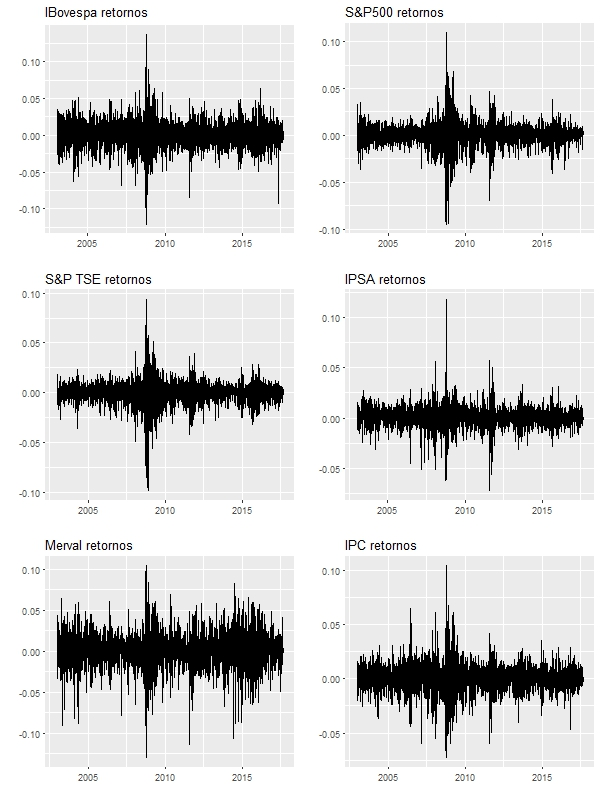
\includegraphics[width=0.9\linewidth]{figs/artigo-retornos}
	\caption{Retornos dos índices do estudo. Período completo entre 01/01/2003 a 30/08/2017.}
	\label{fig:artigo-retornos}
\end{figure}

\begin{figure}[H]
	\centering
	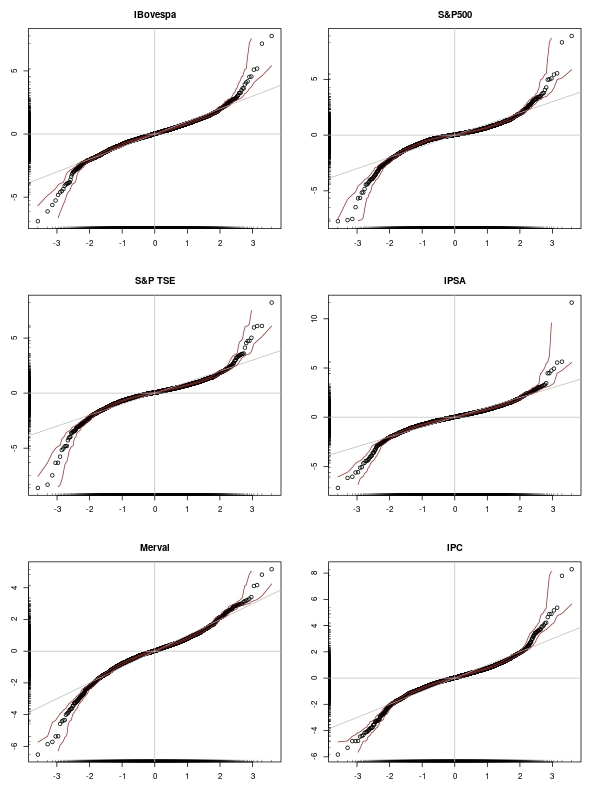
\includegraphics[width=0.9\linewidth]{figs/artigo-qqplots}
	\caption{Análise de normalidade dos retornos através de gráficos quantil-quantil.}
	\label{fig:artigo-qqplots}
\end{figure}

\subsection{Filtro eGARCH}
\label{sec:filtro}

Voltando-se para o período dentro da amostra, o filtro proposto eGARCH(2,1) foi aplicado a estas séries, agora nas perdas que nada mais são que os retornos com o sinal trocado, e seus coeficientes estimados conforme a tabela \ref{tab:garchcoef}. Os valores \emph{p} de cada um destes coeficientes estão apresentados entre parênteses e foram calculados com base em erros-padrão robustos, de acordo com \cite{White1982}.

Como era de se esperar, nem todos os coeficientes estimados são significativos ao nível de confiança de 5\% (alguns nem mesmo a 10\%), o que não invalida o modelo, sendo que para alguns índices específicos talvez fosse possível encontrar outro modelo GARCH mais adequado. A principal função do modelo eGARCH neste primeiro estágio, deve ser lembrado, é a filtragem da série de perdas, de modo que os resíduos padronizados resultantes não sejam autocorrelacionados e tampouco possuam heterocedasticidade. E neste ponto o modelo eGARCH(2,1) se saiu muito bem para todas as séries, conforme demonstrado através dos gráficos de autocorrelação nas figuras \ref{fig:artigo-acf-ibovespa} a \ref{fig:artigo-acf-sptse}.

% latex table generated in R 3.4.3 by xtable 1.8-2 package
% Mon Dec 11 22:38:04 2017
\begin{table}[H]
\centering
\caption{Par\^ametros estimados do modelo eGARCH. Valores p apresentados 
               de acordo com erros padrão robustos. (amostra de trabalho entre 31/08/2003 a 31/08/2013).} 
\label{tab:garchcoef}
\begin{tabular}{lrrrrrr}
  \hline
Parâmetros & IBovespa & S\&P500 & S\&P TSE & IPSA & Merval & IPC \\ 
  \hline
$\mu$ & -0.02941 & -0.02408 & -0.02803 & -0.04435 & -0.08437 & -0.04635 \\ 
   & 0.33805 & 0.08301 & 0.06285 & 0.07210 & 0.04481 & 0.01553 \\ 
  $\phi_1$ & 0.00341 & -0.06726 & 0.00745 & 0.18051 & 0.02976 & 0.05380 \\ 
   & 0.84146 & 0.00017 & 0.70981 & 0.00000 & 0.16595 & 0.00078 \\ 
  $\omega$ & 0.02119 & -0.00233 & -0.00322 & -0.01159 & 0.04476 & 0.00660 \\ 
   & 0.00000 & 0.54715 & 0.29693 & 0.05213 & 0.50349 & 0.02781 \\ 
  $\alpha_1$ & 0.22198 & 0.28021 & 0.19909 & 0.18509 & 0.15027 & 0.16203 \\ 
   & 0.00000 & 0.00000 & 0.00000 & 0.00000 & 0.00002 & 0.00000 \\ 
  $\alpha_2$ & -0.13750 & -0.13789 & -0.11185 & -0.08908 & -0.10071 & -0.06358 \\ 
   & 0.00001 & 0.00030 & 0.00042 & 0.00283 & 0.04321 & 0.02877 \\ 
  $\beta_1$ & 0.97812 & 0.98106 & 0.98309 & 0.95718 & 0.95878 & 0.97938 \\ 
   & 0.00000 & 0.00000 & 0.00000 & 0.00000 & 0.00000 & 0.00000 \\ 
  $\gamma_1$ & -0.05129 & -0.19778 & -0.04319 & 0.19183 & 0.05298 & 0.03944 \\ 
   & 0.29514 & 0.00007 & 0.38635 & 0.00013 & 0.38739 & 0.11206 \\ 
  $\gamma_2$ & 0.19217 & 0.32411 & 0.17950 & 0.04302 & 0.13407 & 0.12604 \\ 
   & 0.00008 & 0.00000 & 0.00026 & 0.36398 & 0.20329 & 0.00003 \\ 
  $\zeta$ & 1.10357 & 1.18792 & 1.24013 & 1.05445 & 1.09390 & 1.16005 \\ 
   & 0.00000 & 0.00000 & 0.00000 & 0.00000 & 0.00000 & 0.00000 \\ 
  $\nu$ & 12.94213 & 7.62352 & 11.77302 & 11.79185 & 5.99271 & 9.13938 \\ 
   & 0.00001 & 0.00000 & 0.00000 & 0.00000 & 0.00000 & 0.00000 \\ 
   \hline
\end{tabular}
\end{table}


Para trabalhar com o \emph{VaR} em seus quantis altos e portanto, modelar a cauda direita da distribuição, passa-se a trabalhar com a distribuição das perdas dos ativos, como alertado anteriormente. Os gráficos ACF são para as distribuições de perdas e seus quadrados na parte superior, e na parte inferior os correlogramas são apresentados para os resíduos padronizados e seus quadrados oriundos do modelo eGARCH. Através destes gráficos fica bastante evidente como a filtragem foi bem sucedida em retirar a autocorrelação encontrada originalmente nas perdas, especialmente em seus quadrados, que demonstra claramente a natureza heterocedástica das séries sob análise. 

% Figuras com os gráficos ACF antes e depois da filtragem eGARCH
\begin{figure}[H]
	\centering
	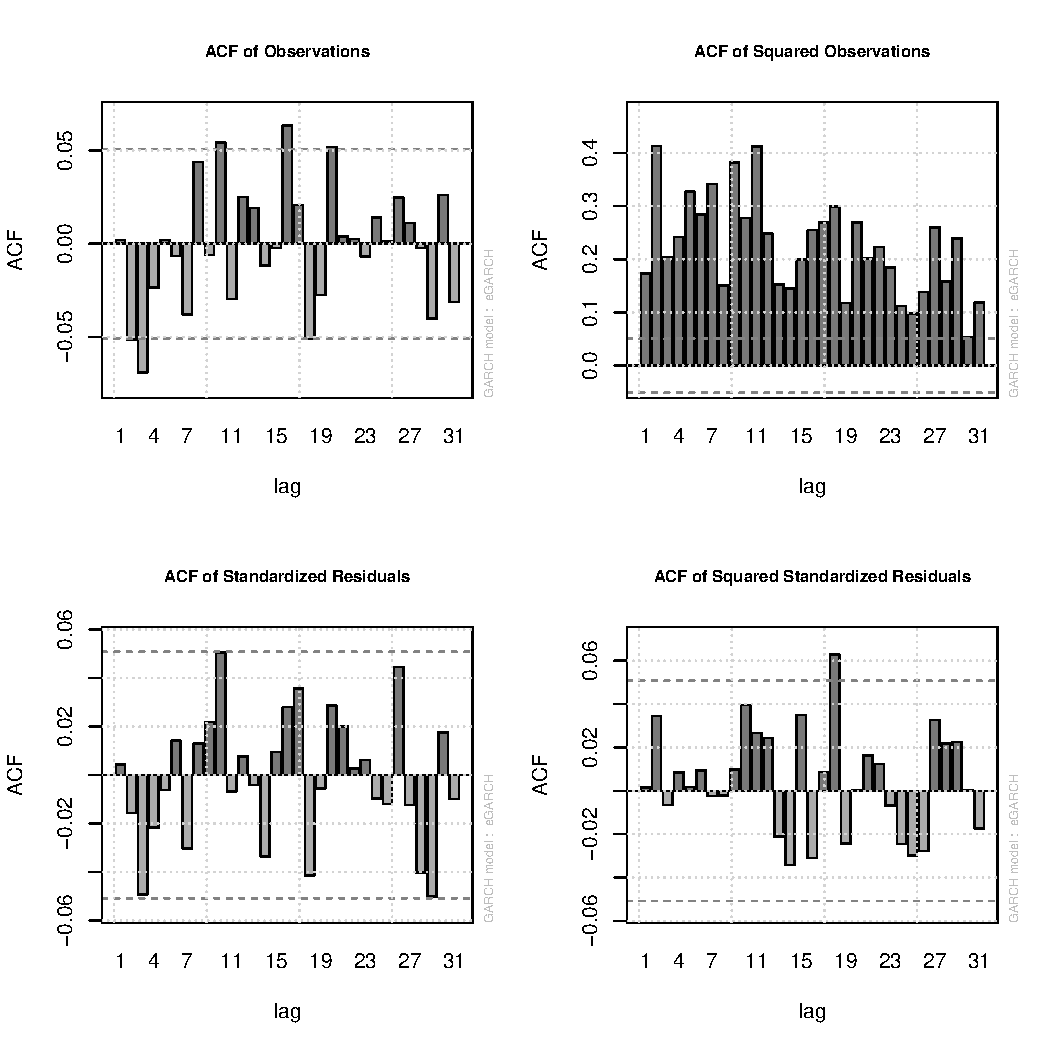
\includegraphics[width=0.9\linewidth]{figs/artigo-acf-IBovespa}
	\caption{Ibovespa. Na parte superior está o ACF das perdas observadas e seus quadrados, enquanto que na parte inferior os resíduos padronizados e seus quadrados após a modelagem eGARCH. Período dentro da amostra 01/01/2013 a 31/12/2008.}
	\label{fig:artigo-acf-ibovespa}
\end{figure}

\begin{figure}[H]
	\centering
	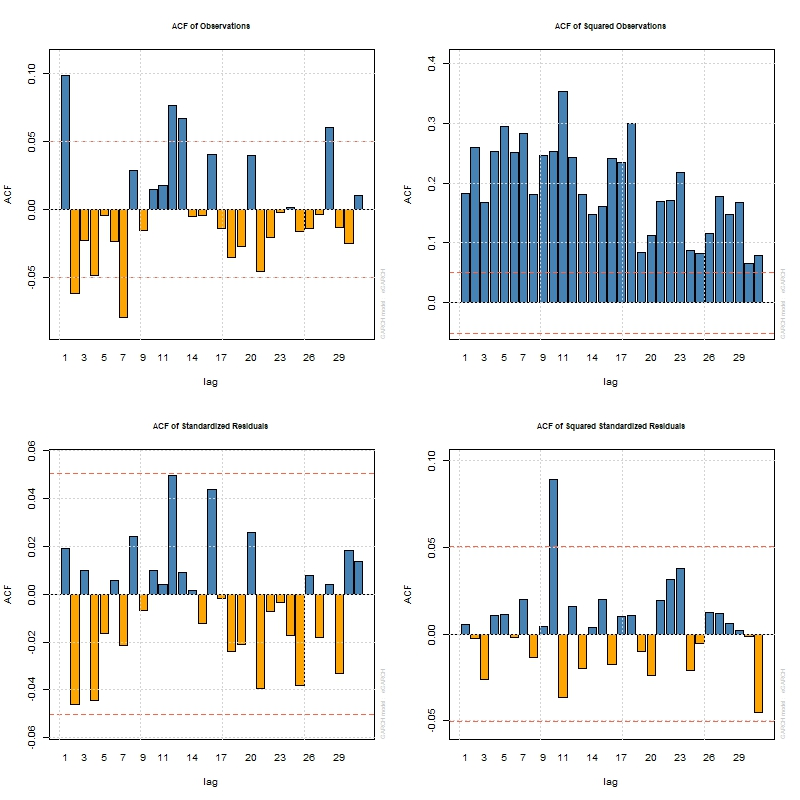
\includegraphics[width=0.9\linewidth]{figs/artigo-acf-IPC}
	\caption{IPC. Na parte superior está o ACF das perdas observadas e seus quadrados, enquanto que na parte inferior os resíduos padronizados e seus quadrados após a modelagem eGARCH. Período dentro da amostra 01/01/2013 a 31/12/2008.}
	\label{fig:artigo-acf-ipc}
\end{figure}

\begin{figure}[H]
	\centering
	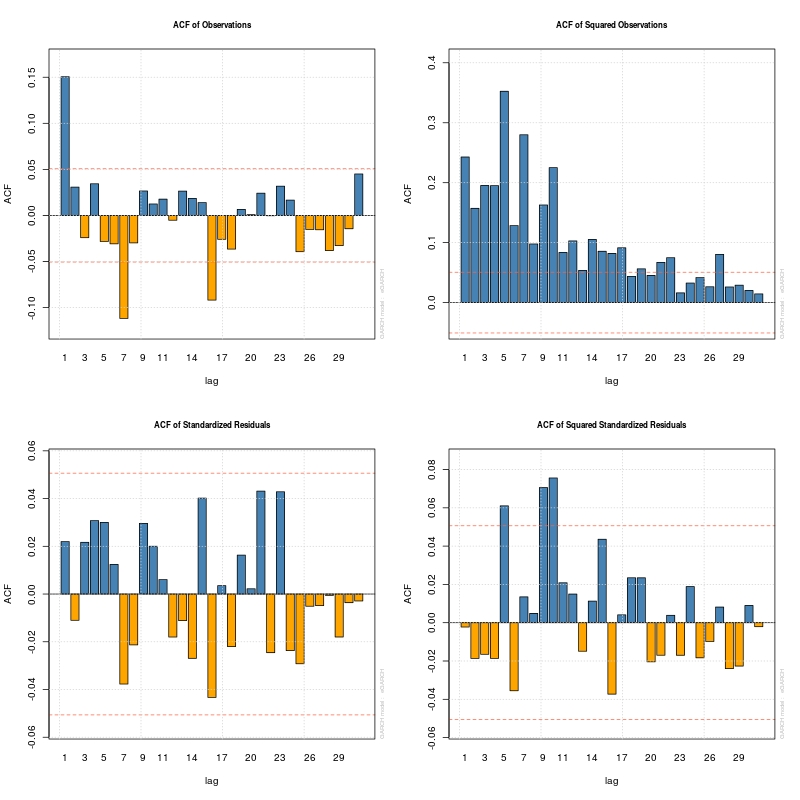
\includegraphics[width=0.9\linewidth]{figs/artigo-acf-IPSA}
	\caption{IPSA. Na parte superior está o ACF das perdas observadas e seus quadrados, enquanto que na parte inferior os resíduos padronizados e seus quadrados após a modelagem eGARCH. Período dentro da amostra 01/01/2013 a 31/12/2008.}
	\label{fig:artigo-acf-ipsa}
\end{figure}

\begin{figure}[H]
	\centering
	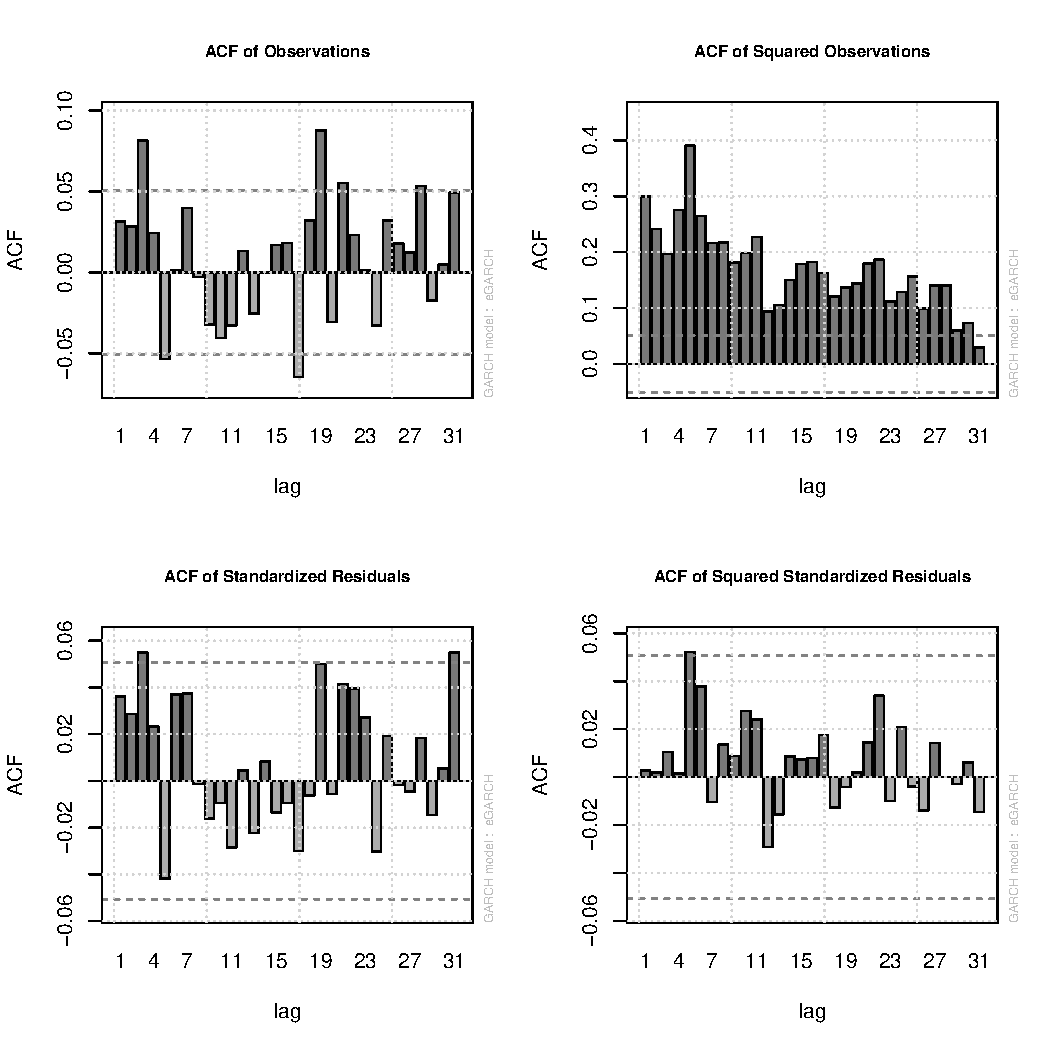
\includegraphics[width=0.9\linewidth]{figs/artigo-acf-Merval}
	\caption{Merval. Na parte superior está o ACF das perdas observadas e seus quadrados, enquanto que na parte inferior os resíduos padronizados e seus quadrados após a modelagem eGARCH. Período dentro da amostra 01/01/2013 a 31/12/2008.}
	\label{fig:artigo-acf-merval}
\end{figure}

\begin{figure}[H]
	\centering
	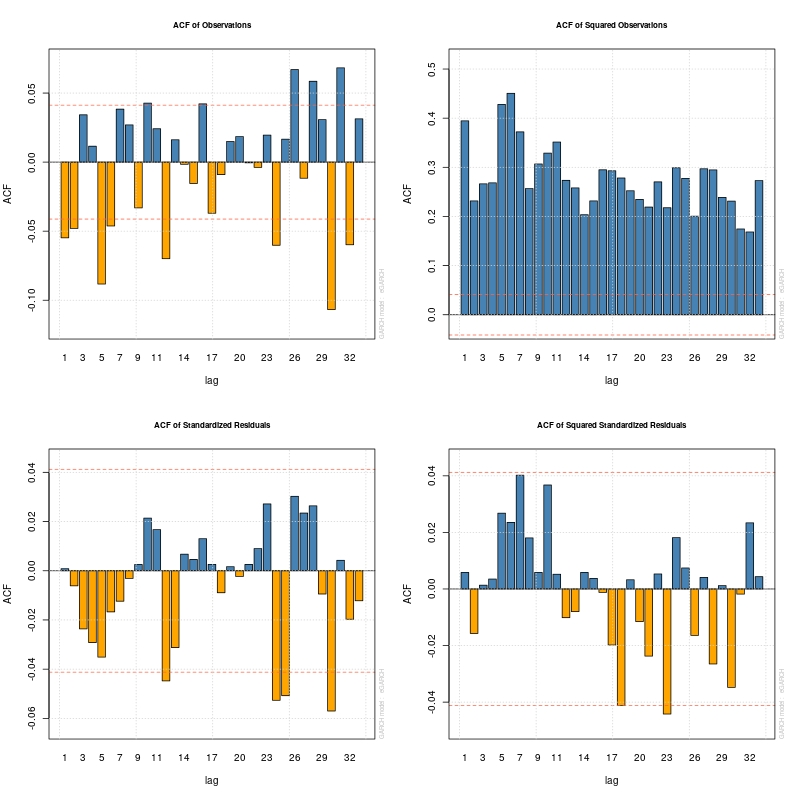
\includegraphics[width=0.9\linewidth]{figs/artigo-acf-SP-TSE}
	\caption{S\&P TSE. Na parte superior está o ACF das perdas observadas e seus quadrados, enquanto que na parte inferior os resíduos padronizados e seus quadrados após a modelagem eGARCH. Período dentro da amostra 01/01/2013 a 31/12/2008.}
	\label{fig:artigo-acf-sptse}
\end{figure}

\begin{figure}[H]
	\centering
	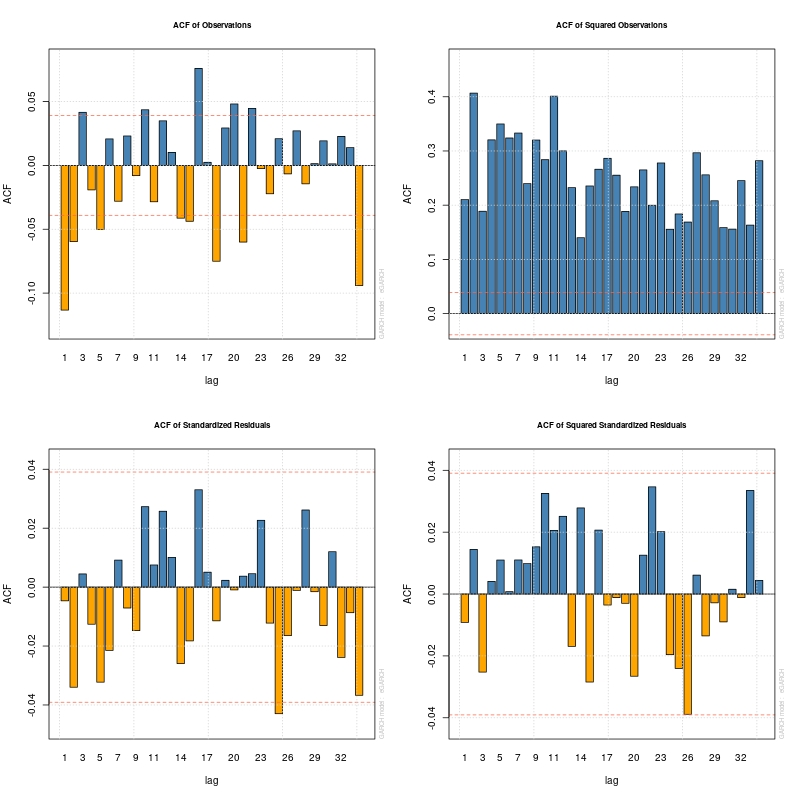
\includegraphics[width=0.9\linewidth]{figs/artigo-acf-SP500}
	\caption{S\&P500. Na parte superior está o ACF das perdas observadas e seus quadrados, enquanto que na parte inferior os resíduos padronizados e seus quadrados após a modelagem eGARCH. Período dentro da amostra 01/01/2013 a 31/12/2008.}
	\label{fig:artigo-acf-sp500}
\end{figure}

A tabela \ref{tab:garchstats} apresenta novamente as estatísticas Jarque-Bera e Ljung-Box (Q e $Q^2$) desta vez para os resíduos padronizados resultantes da filtragem das perdas no primeiro estágio do modelo eGARCH-POT. Enquanto que os resíduos padronizados, assim como os retornos (e as perdas), de fato não são normais como já se esperava, as estatísticas de autocorrelação agora estão todas em favor da ausência desta. Para todos os índices analisados, não é possível rejeitar $H_0$ nos testes de autocorrelação, tanto para os resíduos ($Q(10)$) como para os seus quadrados ($Q^2(10)$) em evidente contraste com os valores apresentados na tabela \ref{tab:descritivas} quando foram analisados os retornos destes índices.

% latex table generated in R 3.4.1 by xtable 1.8-2 package
% Thu Dec 21 19:18:43 2017
\begin{table}[H]
\centering
\caption{Estat�sticas de diagn�stico para o modelo eGARCH. 
               (amostra de trabalho entre 01/01/2003 a 31/12/2008 ).} 
\label{tab:garchstats}
\begin{tabular}{lrrrrrr}
  \hline
Estat�stica & IBovespa & S\&P500 & S\&P TSE & IPSA & Merval & IPC \\ 
  \hline
Jarque-Bera & 49.43583 & 215.01376 & 140.05041 & 34.73241 & 745.12915 & 110.65501 \\ 
   & 0.00000 & 0.00000 & 0.00000 & 0.00000 & 0.00000 & 0.00000 \\ 
  Q(10) & 5.06861 & 6.62418 & 2.48467 & 4.76916 & 10.79623 & 6.51737 \\ 
   & 0.49583 & 0.29224 & 0.88747 & 0.54185 & 0.04803 & 0.30402 \\ 
  $Q^2(10)$ & 2.06336 & 4.68145 & 4.45030 & 7.97618 & 3.96265 & 2.65360 \\ 
   & 0.93211 & 0.55561 & 0.59236 & 0.17130 & 0.67109 & 0.86672 \\ 
   \hline
\end{tabular}
\end{table}


Sendo assim, com retornos padronizados que não são normalmente distribuídos e possuem cauda longas com excesso de curtose, mas que após filtragem não apresentam mais autocorrelação ou heterocedasticidade, pode-se passar ao segundo estágio do model eGARCH-POT, ou seja, aplicar a teoria do valor extremo através do método \emph{peaks over treshold} para parametrizar a cauda direita das distribuições de perdas dos ativos.

\subsection{Método POT}
\label{sec:metpot}

Os resíduos padronizados são tratados como as realizações do processo de inovação no modelo eGARCH(2,1). Estas inovações serão então analisadas sob a ótica da EVT para a obtenção dos parâmetros da GPD que definem a cauda direita de sua distribuição.

Para tanto, deve ser estabelecido um limiar \emph{u} adequado para cada uma das séries, de modo que seja satisfeito o teorema de Pickands-Balkema-de Haan. Este valor de limiar será diferente para cada série e sua escolha deve seguir os princípios delineados na seção \ref{sec:excess} através da função média dos excessos. Entretanto, considerando o \emph{trade-off} existente entre o viés e a variância dos parâmetros estimados da GPD com relação a escolha do valor deste limiar, pode-se abordar o problema desta escolha de outra forma.

Neste artigo foi utilizado o quantil empírico a 92\% para a escolha do valor do limiar. Conforme visto anteriormente, um valor de limiar que resulte em um número de excessos observados a este limiar ($N_u$) entre 100 e 130 parece ser o limiar ótimo a ser escolhido. Considerando o tamanho da janela de dados dentro da amostra para os índices sob análise, este quantil resulta em número de excessos nesta magnitude.

A escolha do limiar através de um quantil empírico fixo também é mais adequada considerando-se que para a fase de \emph{backtesting} do modelo é necessário reavaliar o valo deste limiar para cada dia dentro do período fora da amostra, o que se tornaria inviável de ser feito através da análise gráfica da função média dos excessos.

Escolhido o limiar \emph{u}, trata-se de obter a série de inovações em excesso ao limiar $Z^u_t:{Z^u_t = Z_t-u |Z_t > u}$, onde $Z_t$ são as inovações, em que os resíduos padronizados encontrados são as realizações desta e $Z^u_t$ são portanto, as inovações em excesso, conforme teorizado na seção \ref{sec:var}.

A esta série de inovações em excesso é aplicada a função log-verossimilhança dada em \eqref{eq:gpdloglik} que por sua vez é maximizada em relação aos parâmetros da GPD, $\xi$ e $\psi$, para a obtenção de suas estimativas.

A tabela \ref{tab:evtcoef} apresenta os valores destes parâmetros e seus erros padrão para cada um dos índices, com a estimação feita com os dados do período dentro da amostra. Também são apresentados o número de observações dentro da amostra para o total dos resíduos padronizados, assim como o número de excessos observados ($N_u$) para o limiar escolhido ($u$). Observa-se como o número de excessos varia de acordo com o índice (asim como o total de observações), porém todos ficam em torno de 120 excessos, que é considerado um valor ideal. 

% latex table generated in R 3.4.2 by xtable 1.8-2 package
% Mon Jan  1 13:31:10 2018
\begin{table}[H]
\centering
\caption{Parâmetros estimados para o modelo EVT dos resíduos padronizados. 
               (amostra de trabalho entre 01/01/2003 a 31/12/2008 ).} 
\label{tab:evtcoef}
\begin{tabular}{lrrrrrr}
  \hline
 & IBovespa & S\&P500 & S\&P TSE & IPSA & Merval & IPC \\ 
  \hline
Obs. dentro amostra & 1487.00000 & 1511.00000 & 1522.00000 & 1498.00000 & 1495.00000 & 1514.00000 \\ 
  Limiar & 1.43392 & 1.36357 & 1.48743 & 1.40436 & 1.35673 & 1.40554 \\ 
  Número de excessos & 119.00000 & 121.00000 & 122.00000 & 120.00000 & 120.00000 & 122.00000 \\ 
  Parâmetro forma GPD & -0.01136 & -0.02867 & -0.00749 & 0.00343 & 0.07085 & 0.00287 \\ 
  Erro padrão & 0.07900 & 0.06368 & 0.08595 & 0.08475 & 0.08132 & 0.08418 \\ 
  Parâmetro escala GPD & 0.55190 & 0.72245 & 0.61939 & 0.55517 & 0.65097 & 0.61094 \\ 
  Erro padrão & 0.06679 & 0.08017 & 0.07732 & 0.06915 & 0.07947 & 0.07552 \\ 
  Quantil 97.5\% & 2.07183 & 2.19073 & 2.20595 & 2.05214 & 2.14835 & 2.12178 \\ 
  Quantil 99.0\% & 2.56831 & 2.82263 & 2.76663 & 2.56368 & 2.81771 & 2.68420 \\ 
   \hline
\end{tabular}
\end{table}
	

Na figura \ref{fig:artigo-gpdfit} é possível visualizar os gráficos de ajuste das inovações em excesso de cada um dos índices contra suas distribuições GPD de referência, ou seja, aquelas com os parâmetros de forma e escala estimados para os respectivos índices. Verifica-se que a distribuição destes excessos pouco se desvia com relação a curva de referência, denotando um bom ajuste dos dados ao modelo teórico. Em contraste, quando modelados diretamente através de uma distribuição normal, as séries de retornos se afastavam consideravelmente de suas referências como já apresentado na figura \ref{fig:artigo-qqplots}. Ao se utilizar um método semi-paramétrico como o proposto, modelando apenas uma parte da cauda da distribuição, a parte que interessa para a modelagem de risco, obtém-se uma estimação muito mais próxima da realidade que os dados apresentam.

\begin{figure}[H]
	\centering
	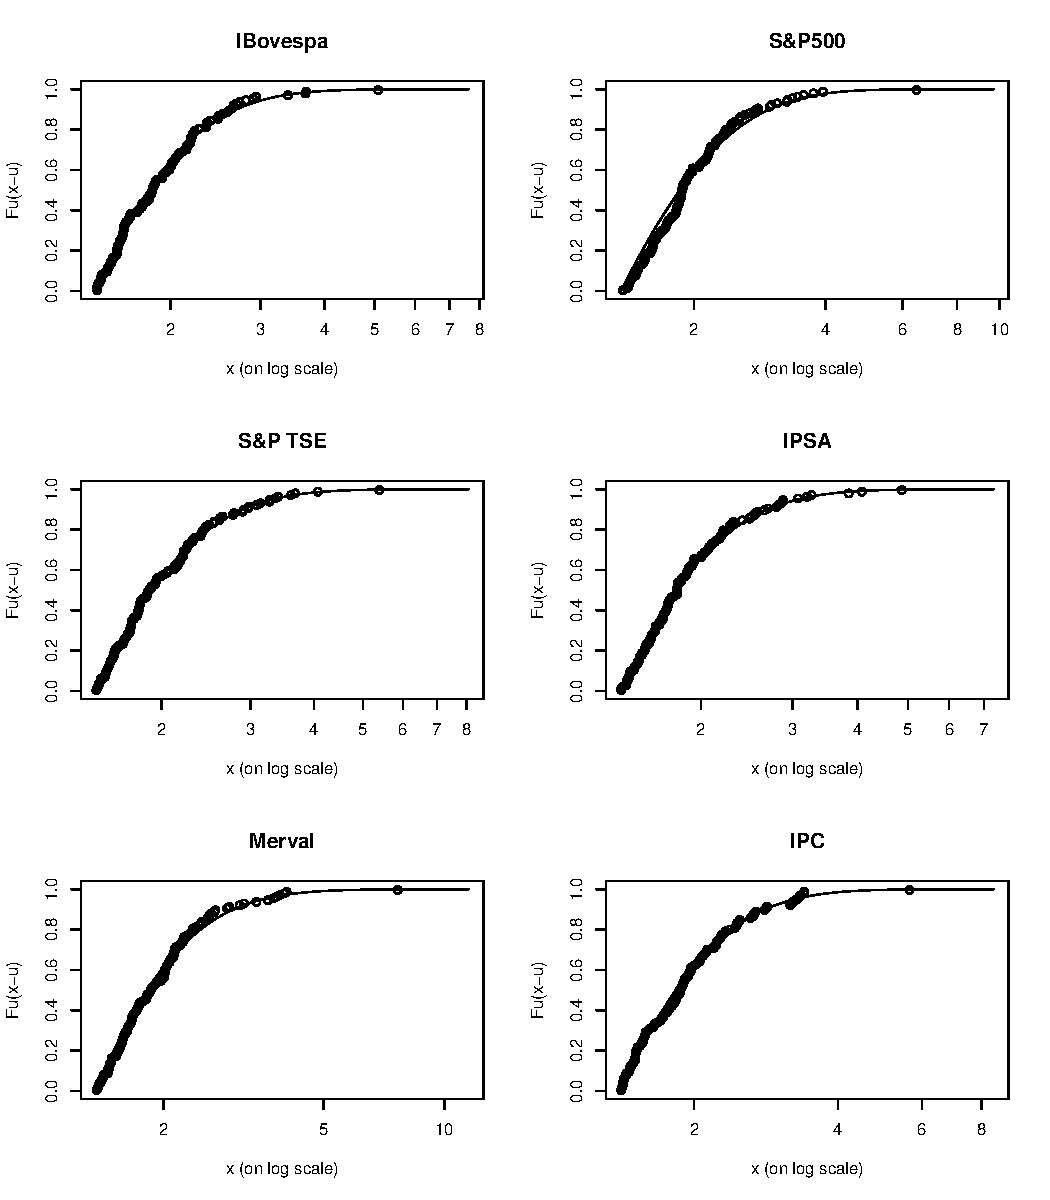
\includegraphics[width=0.9\linewidth]{figs/artigo-gpdfit}
	\caption{Qualidade do ajuste dos dados de inovações em excesso contra uma GPD de referência. Período dentro da amostra.}
	\label{fig:artigo-gpdfit}
\end{figure}

\section{Resultados empíricos}
\label{sec:empiricos}

Os resultados empíricos aqui referidos concentram-se em testar através de \emph{backtest} o modelo EVT condicional apresentado, o qual utiliza a metodologia em dois estágios proposta por \cite{McNeil2000} com um filtro eGARCH(2,1) e o método POT, assim como outros modelos para a estimação do \emph{VaR}, como a Normal e t-Student condicionais, Normal e t-Student incondicionais, o modelo proposto por \cite{RiskMetrics1995} e o próprio modelo EVT incondicional, em um total de sete modelos sendo testados e comparados para fins de estimação da medida de risco.

Para fazer o \emph{backtest}, considere a série $x_1, x_2, \ldots, x_m$, com $m\gg n$ e o conjunto de dias $T = \{n, \ldots, m-1\}$. Uma janela da dados de tamanho fixo $n$ é utilizada e para cada dia $t \in T$ é reestimado o valor de $VaR^t_\alpha$. O período de teste fora da amostra vai de 01/01/2009 a 30/08/2017, com dados diários para as perdas dos índices sob análise. O número de observações ($n$) dentro da janela de dados utilizada para fazer a estimação dos modelos para cada um dos índices é aquele apresentado na tabela \ref{tab:evtcoef} (N.obs.), esse valor é fixo para cada série. Portanto, a partir do início do período de teste, esta janela fixa avança um dia e o modelo é estimado, resultando, com auxílio da equação \eqref{eq:varcond}, no valor estimado de $VaR_\alpha^t$, ou seja, a medida de risco calculada ao final do dia $t$ que deverá ser comparada a perda incorrida no dia a frente, $t+1$.

O quantil para a definição do limiar \emph{u} é fixo em 0,92, o que resultará em valores distintos de limiar para cada rodada do teste, e possivelmente um número diferente de excessos observados. Entretanto essas diferenças, considerando o tamanho fixo da janela de dados, será muito pequeno em torno de uma unidade apenas. Mantém-se assim, um número de excessos em torno de 120 observações, valor adequado para se fazer as estimativas dos parâmetros da GPD.

A figura \ref{fig:artigo-sp500backtest} apresenta o resultado do \emph{backtest} para dois modelos, EVT condicional e normal incondicional. Entende-se por modelos incondicionais aqueles em que a volatilidade histórica de toda a janela de dados é utilizada para calcular as medias de risco. Claramente se percebe como o modelo condicional, que utiliza a última estimação para a volatilidade dos resíduos padronizados e então escalá-los para obter a medida de risco, é muito mais responsivo a alterações no regime de volatilidade do ativo. Um modelo incondicional, por sua vez, não responde de forma acentuada a variações de curto-prazo na volatilidade do ativo, pois estas observações mais extremas são atenuadas em meio a todas as outras observações utilizadas da janela de dados.

\begin{figure}[H]
	\centering
	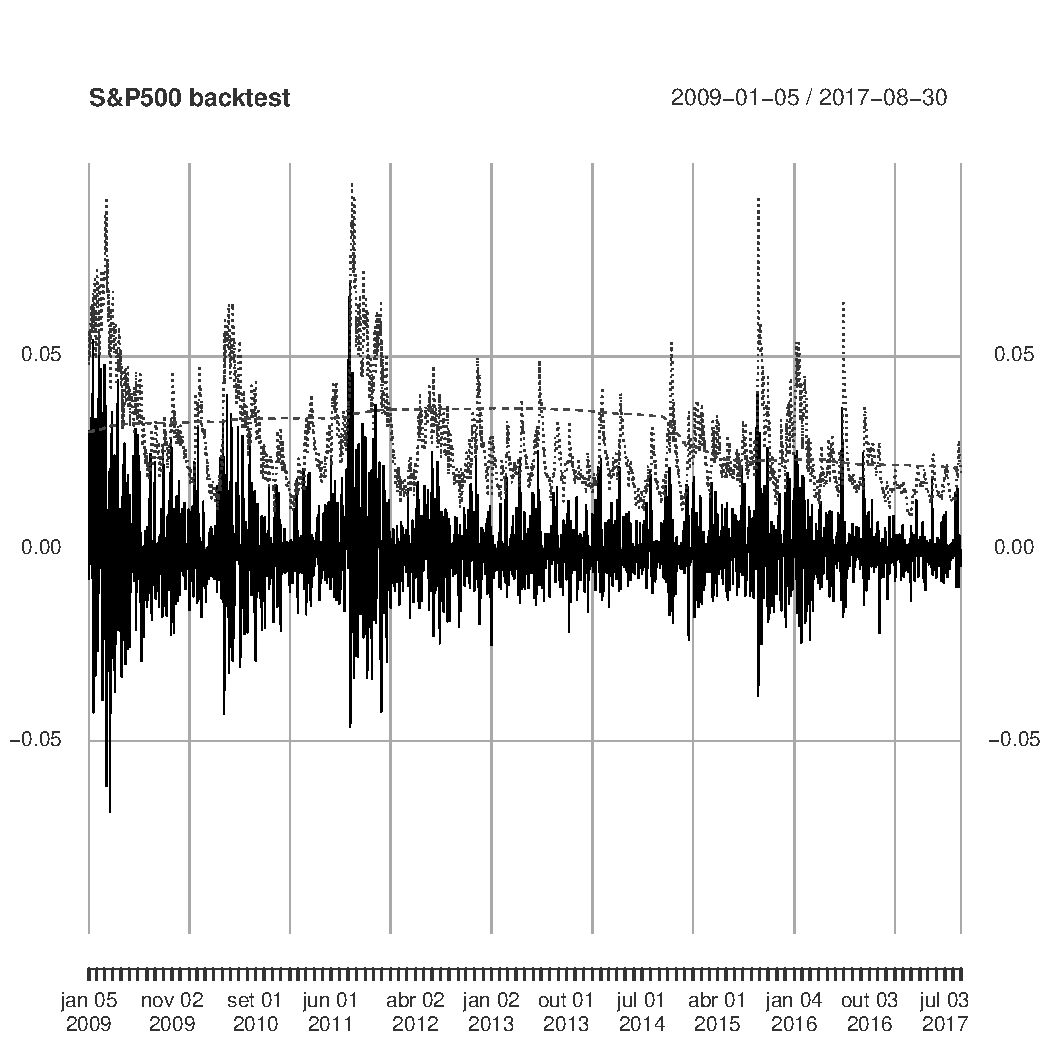
\includegraphics[width=0.9\linewidth]{figs/artigo-sp500backtest}
	\caption{Teste fora da amostra para o S\&P500. O modelo EVT condicional (linha pontilhada) é muito mais reativo a mudanças na volatilidade que um modelo normal incondicional (linha tracejada).}
	\label{fig:artigo-sp500backtest}
\end{figure}

Uma violação é dita ocorrida quando a perda observada é maior que a medida de risco estimada no dia anterior, $x_{t+1}>VaR^t_\alpha$ para um $\alpha$ dentro do conjunto de níveis de significância, neste artigo $\alpha \in \{0,975; 0,990\}$. A tabela \ref{tab:varviol} apresenta em termos percentuais as violações ocorridas para cada um dos modelos para os níveis de cobertura dados.

Pode ser realizado um teste estatístico para verificar se o modelo para $VaR^t_\alpha$ foi corretamente especificado, levando-se em consideração o seu nível de cobertura, $1-\alpha$. Em \cite{Kupiec1995}, este tipo de teste é apresentado. Este permite que seja testado se a frequência de violações ao $VaR$ é consistente com o valor esperado destas violações, o nível de cobertura. Sob a hipótese nula de um modelo corretamente especificado o número de violações segue uma distribuição binomial e o teste toma a forma de razão de verossimilhança com a seguinte estatística:

\begin{equation}
	LR_{uc}=-2\ln\left(\frac{(1-p)^{n-X}p^X}{(1-\frac{X}{n})^{n-X}(\frac{X}{n})^X}\right)
\end{equation}
onde $p$ é o nível de cobertura, $n$ é o número de observações do período fora da amostra e $X$ neste caso é o número de violações ocorridas.

Este teste não faz nenhum tipo de assunção, e por conseguinte não testa, a hipótese de independência entre as violações, sendo considerado um teste \emph{incondicional} para o $VaR$.

% latex table generated in R 3.4.1 by xtable 1.8-2 package
% Thu Dec 21 19:19:27 2017
\begin{table}[H]
\centering
\caption{Percentual de viola��es. (fora da amostra, dados entre 02/01/2009 e 31/08/2017} 
\label{tab:varviol}
\begin{tabular}{lrrrrrr}
  \hline
Modelo & IBovespa & IPC & IPSA & Merval & S\&P TSE & S\&P500 \\ 
  \hline
Cobertura = 1\% &  &  &  &  &  &  \\ 
  EVT Condicional & 0.47 & 0.23 & 0.37 & 0.48 & 0.41 & 0.37 \\ 
  Normal Condicional & 0.56 & 0.46 & 0.42 & 1.00 & 0.78 & 0.73 \\ 
  t-Student Condicional & 0.56 & 0.46 & 0.42 & 1.00 & 0.78 & 0.73 \\ 
  RiskMetrics & 0.42 & 0.60 & 0.65 & 0.90 & 1.06 & 0.78 \\ 
  EVT Incond. Filtrada & 0.19 & 0.05 & 0.05 & 0.57 & 0.14 & 0.14 \\ 
  Normal Incondicional & 0.19 & 0.09 & 0.05 & 0.76 & 0.05 & 0.14 \\ 
  t-Student Incondicional & 0.09 & 0.05 & 0.00 & 0.52 & 0.00 & 0.00 \\ 
  Cobertura = 2.5\% &  &  &  &  &  &  \\ 
  EVT Condicional & 0.84 & 0.60 & 0.79 & 1.14 & 0.87 & 0.73 \\ 
  Normal Condicional & 0.98 & 0.92 & 0.88 & 1.33 & 1.47 & 0.92 \\ 
  t-Student Condicional & 0.93 & 0.92 & 0.83 & 1.28 & 1.47 & 0.92 \\ 
  RiskMetrics & 0.98 & 1.29 & 0.93 & 1.28 & 1.66 & 1.24 \\ 
  EVT Incond. Filtrada & 0.56 & 0.14 & 0.09 & 0.95 & 0.41 & 0.32 \\ 
  Normal Incondicional & 0.42 & 0.14 & 0.05 & 1.09 & 0.23 & 0.18 \\ 
  t-Student Incondicional & 0.42 & 0.14 & 0.05 & 1.00 & 0.28 & 0.18 \\ 
   \hline
\end{tabular}
\end{table}


Um teste condicional é aquele proposto, entre outros, por \cite{Christoffersen2004}. A hipótese de independência entre as violações está relacionada a duração entre as observações destas. O tempo que se passa entre uma violação e outra deve ser independente e não formar agrupamentos (\emph{clusters}). Sob a hipótese nula de um modelo corretamente especificado, esta duração não deve possuir memória. Como a única distribuição contínua que não possui memória é a distribuição exponencial, os autores propõe ajustar os dados a uma distribuição Weibull da qual a exponencial é um caso particular quando o parâmetro $b=1$ e, portanto, o teste é feito sobre este parâmetro.

\todo{Verificar codigo VaRDurTest. Esse teste é conjunto ou somente sobre a hipotese de independência?}
\todo{Ler Christoffersen2004 e escrever a equacao da estatística}

\todo{Teste de sign-bias não deu nenhuma rejeicao de H0. Esquecer ou implementar modelos diferentes para cada ativo?}

% latex table generated in R 3.4.3 by xtable 1.8-2 package
% Fri Jan 12 13:52:36 2018
\begin{longtable}{llrrrrrr}
\caption{Testes estatísticos para o VaR. Teste incondicional de Kupiec, \emph{LRuc}, e teste de
             independência por duração de Christoffersen e Pelletier, \emph{LRdur}. Os modelos testados
são: EVT condicional (cevt), Normal condicional (cnorm), t-Student condicional (ct), Riskmetrics 
(riskmetrics), EVT incondicioanl (uevt), Normal incondicional (unorm) e t-Student incondicional (ut). 
(Período fora da amostra entre 02/01/2009 e 30/08/2017).} \\ 
  \hline
Modelo & Estatística & IBovespa & IPC & IPSA & Merval & S\&P TSE & S\&P500 \\ 
  \hline
Cobertura 1\% &  &  &  &  &  &  &  \\ 
  cevt & LRuc & 0.92 & 0.02 & 1.27 & 1.58 & 0.07 & 0.07 \\ 
  cevt & LRuc p-valor & 0.34 & 0.89 & 0.26 & 0.21 & 0.79 & 0.80 \\ 
  cevt & LRdur & 0.98 & 2.04 & 0.29 & 2.34 & 0.37 & 3.92 \\ 
  cevt & LRdur p-valor & 0.32 & 0.15 & 0.59 & 0.13 & 0.54 & 0.05 \\ 
  cnorm & LRuc & 3.78 & 15.16 & 9.15 & 24.00 & 11.22 & 20.57 \\ 
  cnorm & LRuc p-valor & 0.05 & 0.00 & 0.00 & 0.00 & 0.00 & 0.00 \\ 
  cnorm & LRdur & 2.46 & 0.58 & 0.02 & 1.99 & 0.02 & 0.39 \\ 
  cnorm & LRdur p-valor & 0.12 & 0.44 & 0.90 & 0.16 & 0.89 & 0.53 \\ 
  ct & LRuc & 3.78 & 17.94 & 9.15 & 25.66 & 12.43 & 25.32 \\ 
  ct & LRuc p-valor & 0.05 & 0.00 & 0.00 & 0.00 & 0.00 & 0.00 \\ 
  ct & LRdur & 2.46 & 0.66 & 0.02 & 2.94 & 0.00 & 0.19 \\ 
  ct & LRdur p-valor & 0.12 & 0.42 & 0.90 & 0.09 & 0.96 & 0.66 \\ 
  riskmetrics & LRuc & 4.56 & 20.91 & 19.54 & 29.10 & 34.26 & 32.22 \\ 
  riskmetrics & LRuc p-valor & 0.03 & 0.00 & 0.00 & 0.00 & 0.00 & 0.00 \\ 
  riskmetrics & LRdur & 1.05 & 0.07 & 4.93 & 3.16 & 0.00 & 2.11 \\ 
  riskmetrics & LRdur p-valor & 0.31 & 0.79 & 0.03 & 0.08 & 0.98 & 0.15 \\ 
  uevt & LRuc & 1.53 & 4.07 & 1.61 & 0.72 & 0.80 & 2.18 \\ 
  uevt & LRuc p-valor & 0.22 & 0.04 & 0.21 & 0.40 & 0.37 & 0.14 \\ 
  uevt & LRdur & 1.20 & 3.21 & 10.38 & 8.29 & 35.76 & 28.49 \\ 
  uevt & LRdur p-valor & 0.27 & 0.07 & 0.00 & 0.00 & 0.00 & 0.00 \\ 
  unorm & LRuc & 0.59 & 0.66 & 7.85 & 6.82 & 1.67 & 0.77 \\ 
  unorm & LRuc p-valor & 0.44 & 0.42 & 0.01 & 0.01 & 0.20 & 0.38 \\ 
  unorm & LRdur & 2.49 & 9.73 & 7.92 & 4.70 & 40.84 & 31.79 \\ 
  unorm & LRdur p-valor & 0.11 & 0.00 & 0.00 & 0.03 & 0.00 & 0.00 \\ 
  ut & LRuc & 9.33 & 9.57 & 13.51 & 0.41 & 6.54 & 5.32 \\ 
  ut & LRuc p-valor & 0.00 & 0.00 & 0.00 & 0.52 & 0.01 & 0.02 \\ 
  ut & LRdur & 0.52 & 0.66 & 16.16 & 8.62 & 11.24 & 18.50 \\ 
  ut & LRdur p-valor & 0.47 & 0.41 & 0.00 & 0.00 & 0.00 & 0.00 \\ 
  Cobertura 2.5\% &  &  &  &  &  &  &  \\ 
  cevt & LRuc & 0.01 & 0.00 & 0.02 & 1.33 & 0.36 & 0.24 \\ 
  cevt & LRuc p-valor & 0.93 & 0.99 & 0.89 & 0.25 & 0.55 & 0.63 \\ 
  cevt & LRdur & 0.39 & 0.55 & 0.03 & 2.82 & 0.36 & 0.27 \\ 
  cevt & LRdur p-valor & 0.53 & 0.46 & 0.86 & 0.09 & 0.55 & 0.60 \\ 
  cnorm & LRuc & 0.11 & 4.38 & 0.67 & 8.71 & 10.10 & 13.21 \\ 
  cnorm & LRuc p-valor & 0.74 & 0.04 & 0.41 & 0.00 & 0.00 & 0.00 \\ 
  cnorm & LRdur & 0.43 & 0.14 & 0.37 & 0.54 & 0.86 & 0.01 \\ 
  cnorm & LRdur p-valor & 0.51 & 0.71 & 0.55 & 0.46 & 0.35 & 0.92 \\ 
  ct & LRuc & 0.11 & 3.86 & 0.17 & 7.99 & 10.10 & 13.21 \\ 
  ct & LRuc p-valor & 0.74 & 0.05 & 0.68 & 0.00 & 0.00 & 0.00 \\ 
  ct & LRdur & 0.43 & 0.10 & 0.32 & 0.51 & 0.86 & 0.01 \\ 
  ct & LRdur p-valor & 0.51 & 0.75 & 0.57 & 0.48 & 0.35 & 0.92 \\ 
  riskmetrics & LRuc & 4.17 & 8.79 & 5.60 & 6.63 & 21.18 & 23.10 \\ 
  riskmetrics & LRuc p-valor & 0.04 & 0.00 & 0.02 & 0.01 & 0.00 & 0.00 \\ 
  riskmetrics & LRdur & 7.73 & 1.55 & 3.58 & 1.00 & 0.26 & 2.50 \\ 
  riskmetrics & LRdur p-valor & 0.01 & 0.21 & 0.06 & 0.32 & 0.61 & 0.11 \\ 
  uevt & LRuc & 5.90 & 13.12 & 2.95 & 0.00 & 0.05 & 0.39 \\ 
  uevt & LRuc p-valor & 0.02 & 0.00 & 0.09 & 0.95 & 0.82 & 0.53 \\ 
  uevt & LRdur & 16.55 & 14.30 & 20.53 & 6.93 & 30.09 & 42.63 \\ 
  uevt & LRdur p-valor & 0.00 & 0.00 & 0.00 & 0.01 & 0.00 & 0.00 \\ 
  unorm & LRuc & 6.69 & 6.24 & 19.86 & 3.27 & 0.36 & 3.19 \\ 
  unorm & LRuc p-valor & 0.01 & 0.01 & 0.00 & 0.07 & 0.55 & 0.07 \\ 
  unorm & LRdur & 14.09 & 19.01 & 8.98 & 13.89 & 40.84 & 31.24 \\ 
  unorm & LRdur p-valor & 0.00 & 0.00 & 0.00 & 0.00 & 0.00 & 0.00 \\ 
  ut & LRuc & 9.39 & 7.91 & 15.52 & 2.40 & 0.10 & 5.01 \\ 
  ut & LRuc p-valor & 0.00 & 0.00 & 0.00 & 0.12 & 0.75 & 0.03 \\ 
  ut & LRdur & 13.54 & 19.03 & 6.98 & 17.92 & 42.74 & 31.96 \\ 
  ut & LRdur p-valor & 0.00 & 0.00 & 0.01 & 0.00 & 0.00 & 0.00 \\ 
   \hline
\hline
\label{tab:vartest}
\end{longtable}






\section{Conclusão}

\section*{Referências}

\bibliography{library}

\end{document}
